\newpage
\section{Sistema B – Controlo de Climatização}


\begin{figure}[H]
    % \centering
    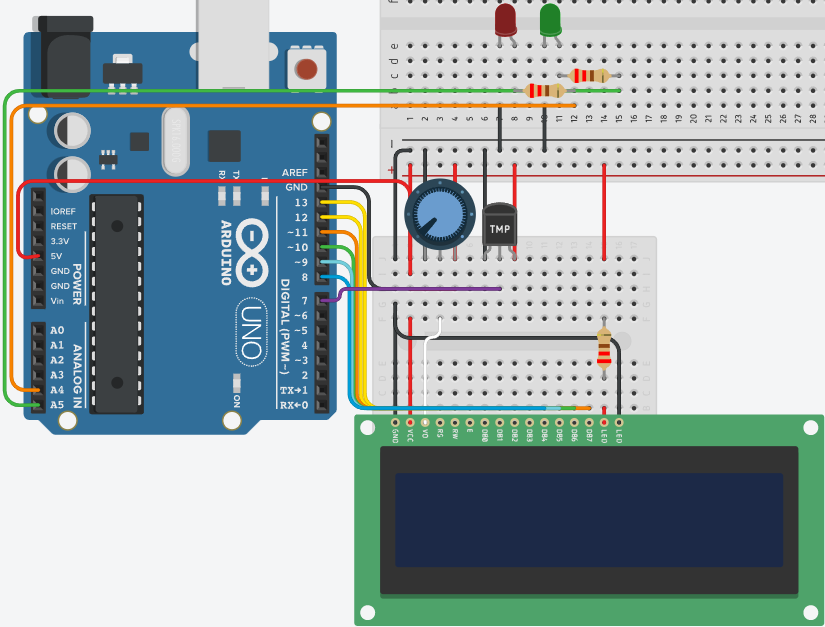
\includegraphics[scale=0.5]{images/hardware/sisB_tinkercad.png}
    \selectlanguage{portuguese}\caption{Esquema do Sistema}
\end{figure}
% A solução deste sistema exige a utilização de:
\begin{table}[H]
    \centering
    \setlength{\arrayrulewidth}{0.5mm}
    \renewcommand{\arraystretch}{1.5}
    \begin{tabular}{|l|c|}
        \hline
        \multicolumn{1}{|c|}{Componentes} & \multicolumn{1}{|c|}{Quantidade}\\ [0.8ex] 
        \hline
        Arduino & 1x\\
        \hline
        LCD 16x2 & 1x\\
        \hline
        Potenciómetro 10k$\Omega$ & 1x\\
        \hline
        Sensor de Temperatura DHT11 & 1x\\
        \hline
        LED Vermelho & 1x\\
        \hline
        LED Verde & 1x\\
        \hline
        Resistência 220$\Omega$ & 3x\\
        \hline
    \end{tabular}
    \selectlanguage{portuguese}
    \caption{Lista dos Componentes}
\end{table}

O LCD está ligado à placa Arduino do seguinte modo:\\
(Da esquerda para a direita do LCD)
\begin{itemize}
    \item GCC -- GND
    \item VCC -- 5V
    \item V0 -- Pino Analógico do Potenciómetro
    \item RS -- 13
    \item RW -- GND
    \item E -- 12
    \item D0 > D3 -- Desconectados
    \item D4 -- 8
    \item D5 -- 9
    \item D6 -- 10
    \item D7 -- 11
\end{itemize}

O sensor de temperatura, que no esquema físico corresponde ao modelo DHT11, encontra-se ligado à porta digital n$^{o}$ 7.

Os LED's Verde e Vermelho encontram-se ligados às portas analógicas 5 e 4 respetivamente.